The statistical and systematic uncertainties are treated as nuisance parameters (NP) for
limit computation. The statistical uncertainty is propagated through the \verb|autoMCStats| tool.
Which adds histograms of each individual background process and assigns one nuisance in each bin of
the total background. For each systematic uncertainty, one NP is assigned. There are different types 
of probability distribution function (PDF) associated with each NP that goes in the likelihood for 
limit computation. If for the given NP, the PDF is log-normal (Gaussian) distribution then the 
corresponding NP is said to be profiled as lnN (shape). Since the final observable is $\mjj$, 
a NP is profiled as shape (lnN) based on whether its value is different (same) for all 
the bins of $\mjj$. From Figures~\ref{fig:shapeVslnN1}--\ref{fig:shapeVslnN6}, it can be seen that 
the ratio of up and down template with the base is compatible with a flat line for jet energy scale,
jet energy resolution, \PQb/\PQc tagging, and \PQt quark \pt systematics. Therefore, these NPs are 
profiled as lnN. The trend for \PQt quark mass (\verb|topMass_tt|), renormalization and factorization
scale (\verb|scaleRF_tt|), and parton showering matching (\verb|hDamp_tt|) is mixed. Hence these are 
also, conservatively, profiled as lnN. A description of the acronyms used to denote the NPs is shown 
in Table~\ref{t:npDisc}.
\begin{table}
\caption{ Description of nuisance parameters corresponding to the systematic and statistical
uncertainties.}
\label{t:npDisc}
\begin{center}
\begin{tabular}{ccp{9cm}}
\hline
\hline
{\bf{NP name}} & {\bf{Profile}} & {\bf{NP description}} \\
\hline
\hline
Systematics: & & \\
\verb|lumi_13TeV|     & lnN & uncertainty in the luminosity measurement at 13 \TeV\\
\verb|CMS_eff_l|      & lnN & lepton (\rm{e}, $\mu$) selection uncertainty \\
\verb|CMS_eff_bcInc1| & lnN & uncertainty from inclusive \PQb/\PQc tagging-1 \\
\verb|CMS_eff_bcInc2| & lnN & uncertainty from inclusive \PQb/\PQc tagging-2\\ 
\verb|CMS_eff_bcInc3| & lnN & uncertainty from inclusive \PQb/\PQc tagging-3 \\
\verb|CMS_pileup|     & lnN & uncertainty from pileup reweighting\\
\verb|CMS_scale_j|    & lnN & uncertainty from jet energy scale (JES)\\ 
\verb|CMS_res_j|      & lnN & uncertainty from jet energy resolution (JER)\\ 
\verb|CMS_norm_tt|    & lnN & uncertainty on the \ttjets cross section\\
\verb|CMS_norm_stop|  & lnN & uncertainty on the single \PQt cross section\\
\verb|CMS_norm_wjet|  & lnN & uncertainty on the \wjets cross section\\
\verb|CMS_norm_zjet|  & lnN & uncertainty on the \dyjets cross section\\
\verb|CMS_norm_qcd|   & lnN & uncertainty from the data-driven QCD multijet\\
\verb|CMS_norm_vv|    & lnN & uncertainty on the \text{VV} cross section\\
\verb|CMS_topPtReweight| & lnN & uncertainty from \PQt quark \pt reweighting\\
\verb|scaleRF_tt|     & lnN &  uncertainty from renormalisation (R) and factorization (F) scale\\
\verb|hDamp_tt|       & lnN &  uncertainty from parton-shower matching\\
\verb|topMass_tt|     & lnN &    uncertainty from \PQt mass $\pm$ 1 \GeV\\
\hline
Statistical: & & \\
\verb|prop_binch*bin*| & shape & bin-by-bin statistical uncertainties from \verb|autoMCStats|\\
\hline
\end{tabular}
\end{center}
\end{table}

\newpage
\begin{figure}
    \centering  
    {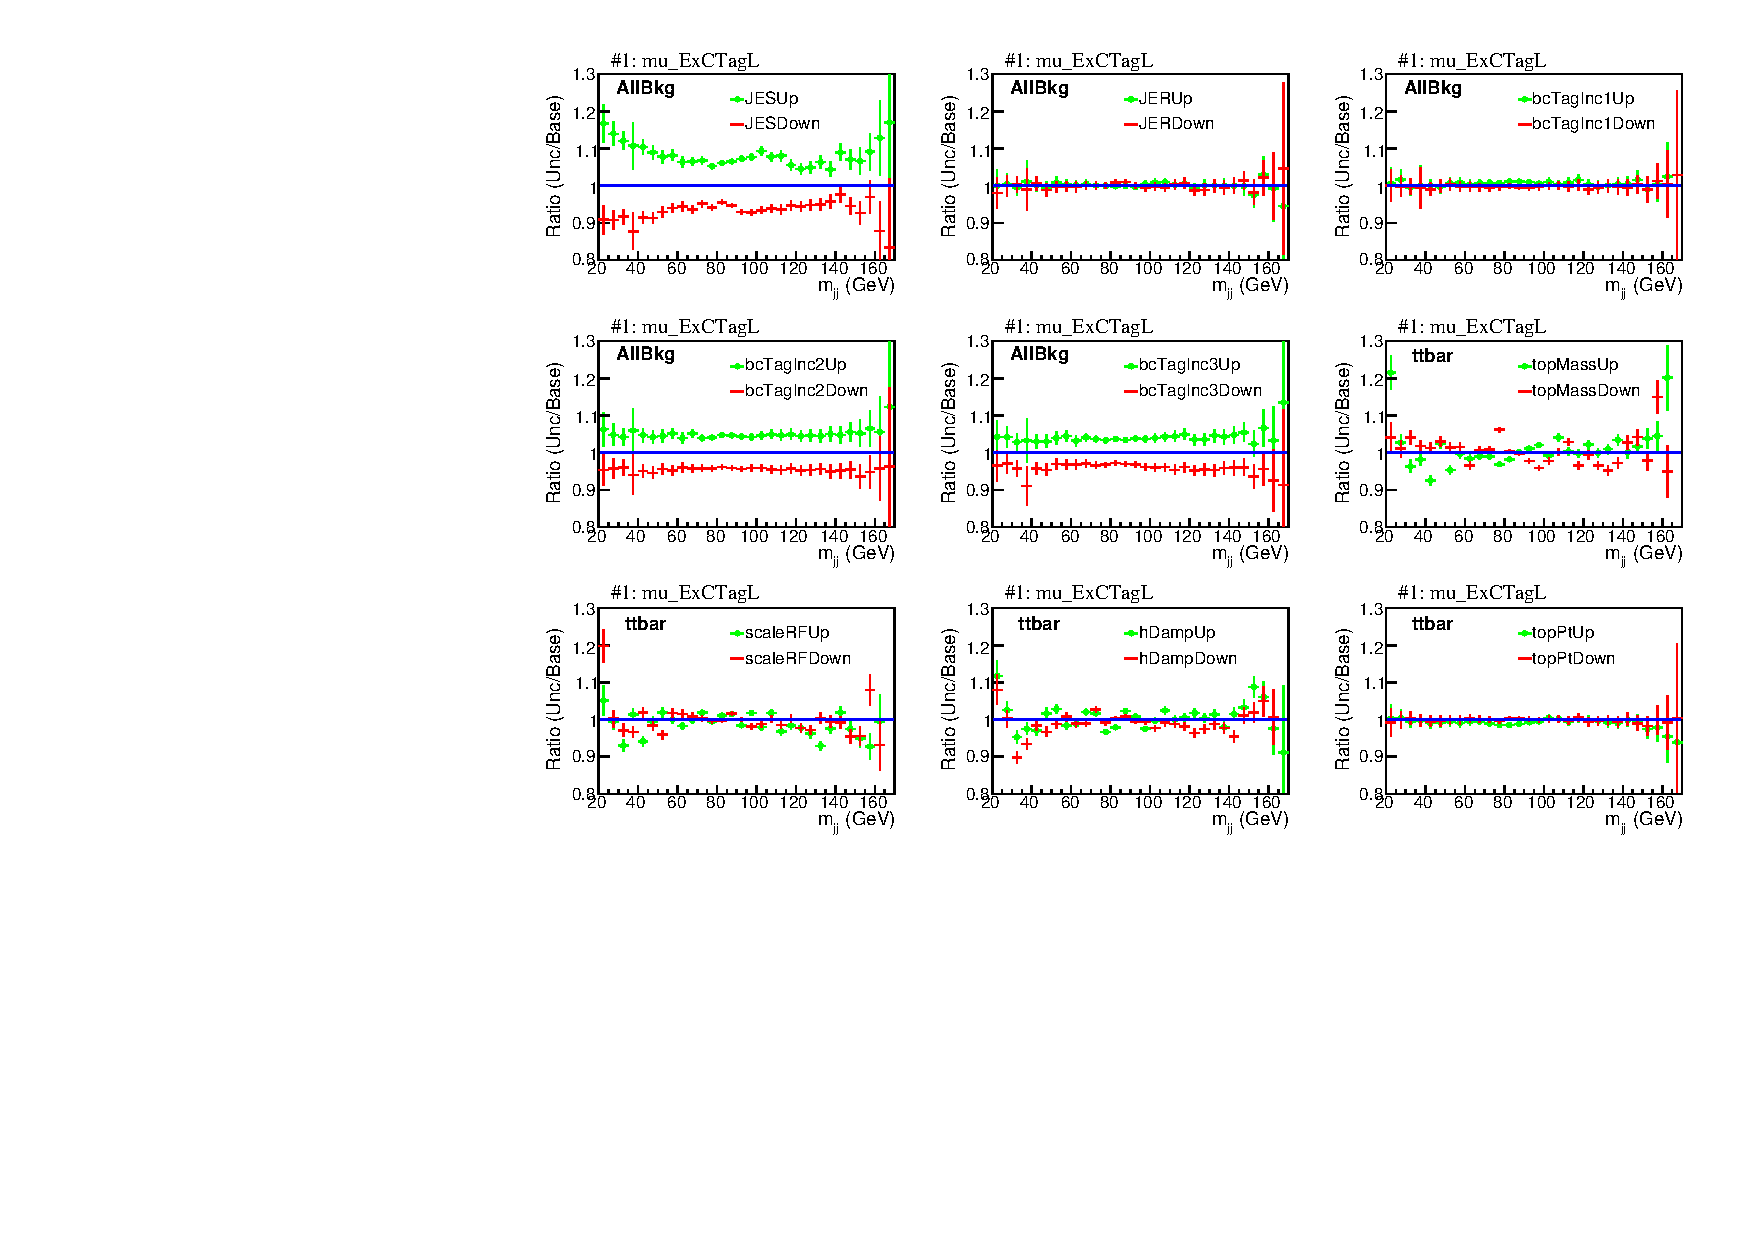
\includegraphics[width=0.80\linewidth]{Image/SYS/RatioBaseSys/mjj_1_mu_ExCTagL.pdf}}
    \caption{ Ratio of up and down with base template for exclusive loose charm category for \mujets channel. }
    \label{fig:shapeVslnN1}
\end{figure}


\begin{figure}
    \centering  
    {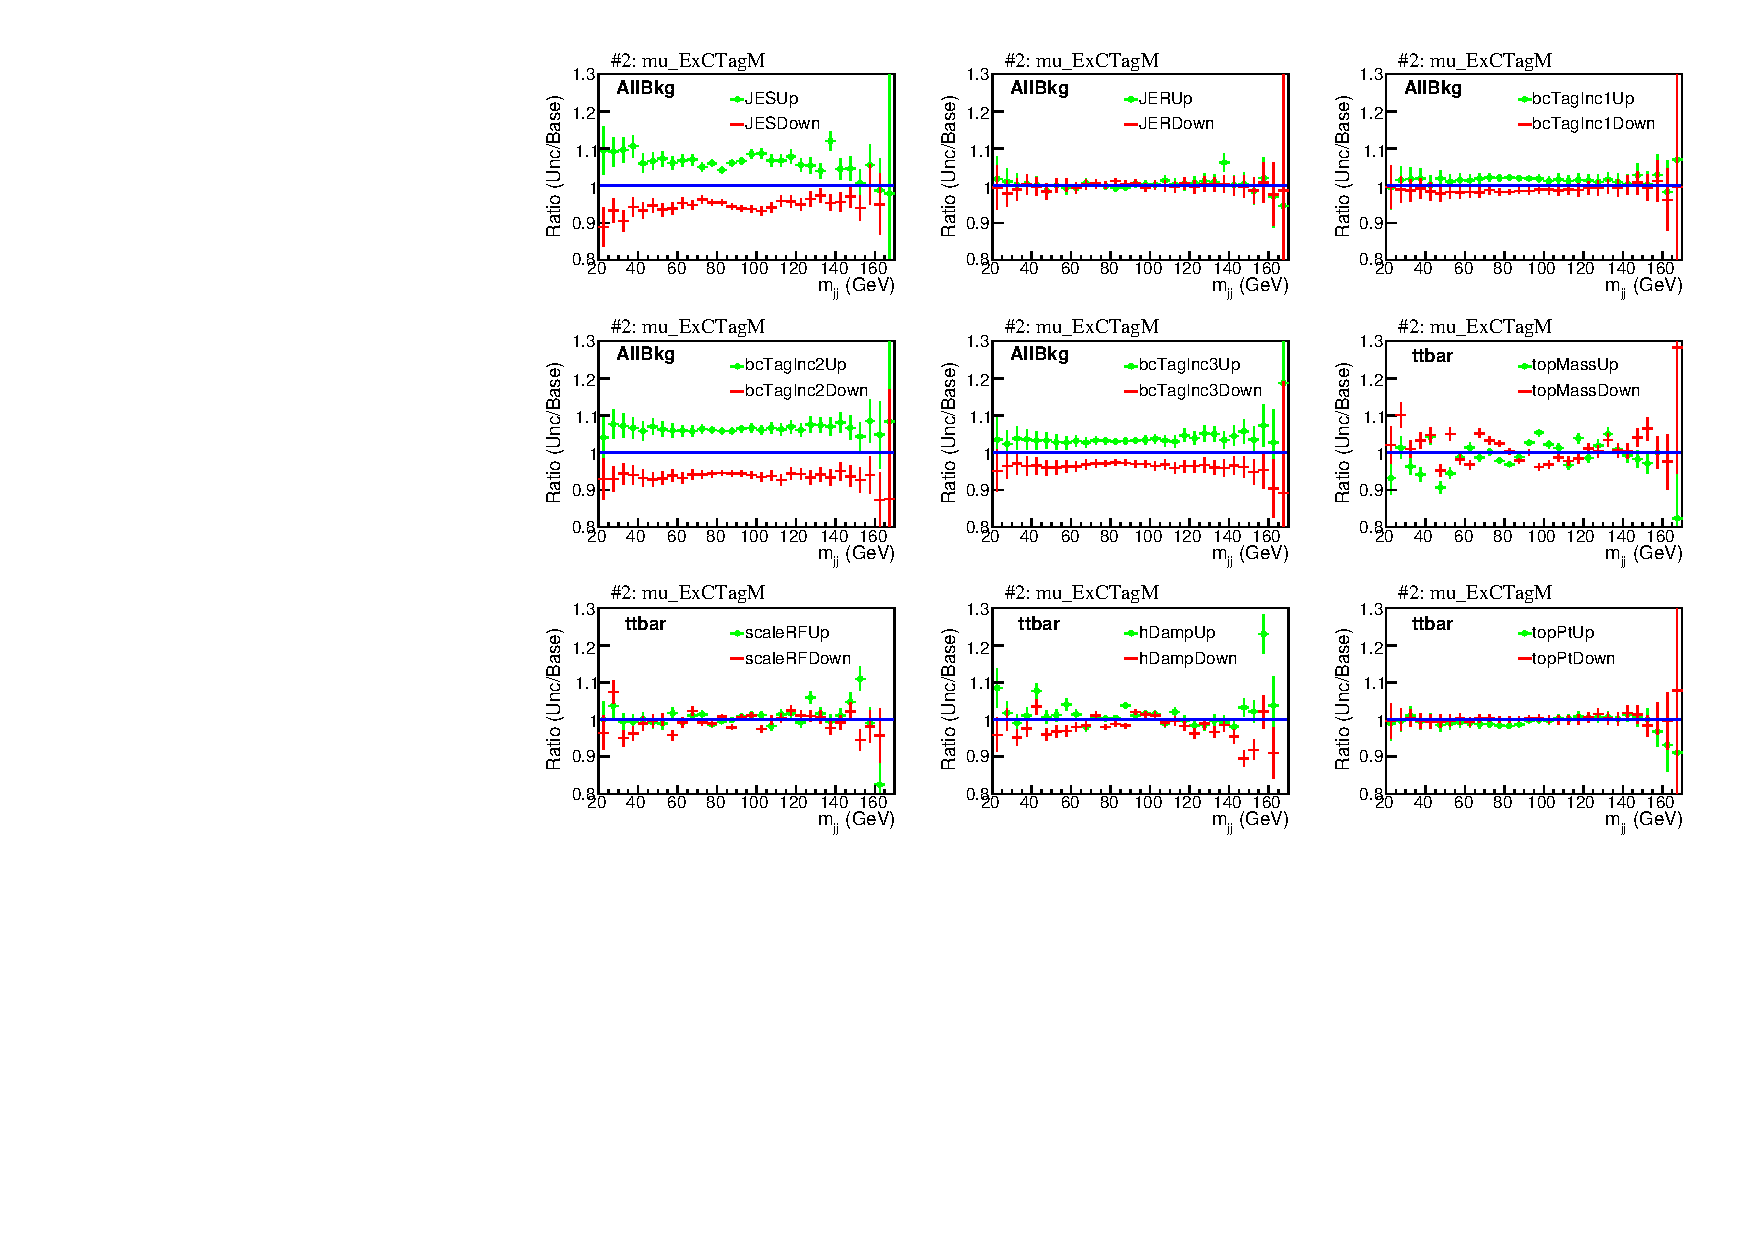
\includegraphics[width=0.80\linewidth]{Image/SYS/RatioBaseSys/mjj_2_mu_ExCTagM.pdf}}
    \caption{ Ratio of up and down with base template for exclusive medium charm category for \mujets channel.}
    \label{fig:shapeVslnN2}
\end{figure}
\begin{figure}
    \centering  
    {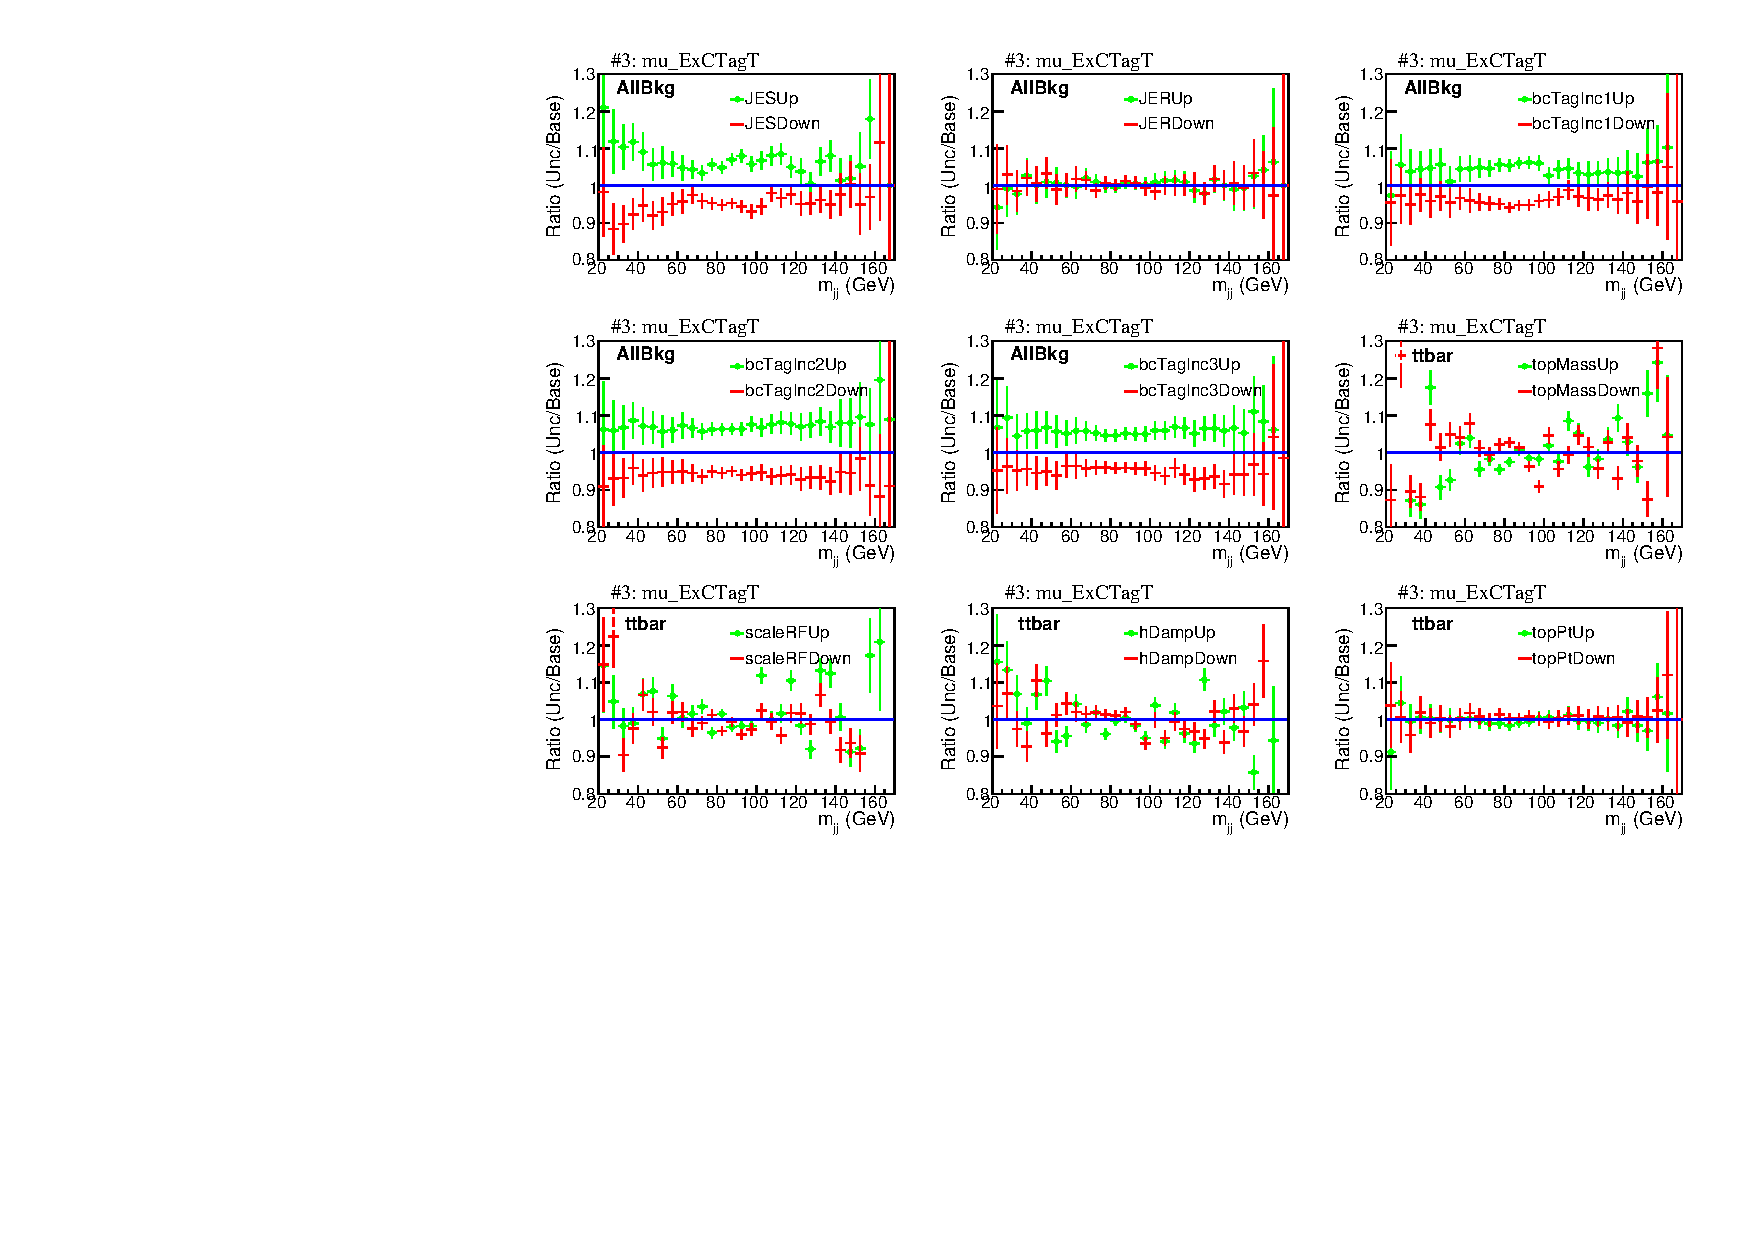
\includegraphics[width=0.80\linewidth]{Image/SYS/RatioBaseSys/mjj_3_mu_ExCTagT.pdf}}
    \caption{ Ratio of up and down with base template from  exclusive tight charm category for \mujets channel. }
    \label{fig:shapeVslnN3}
\end{figure}


\begin{figure}
    \centering  
    {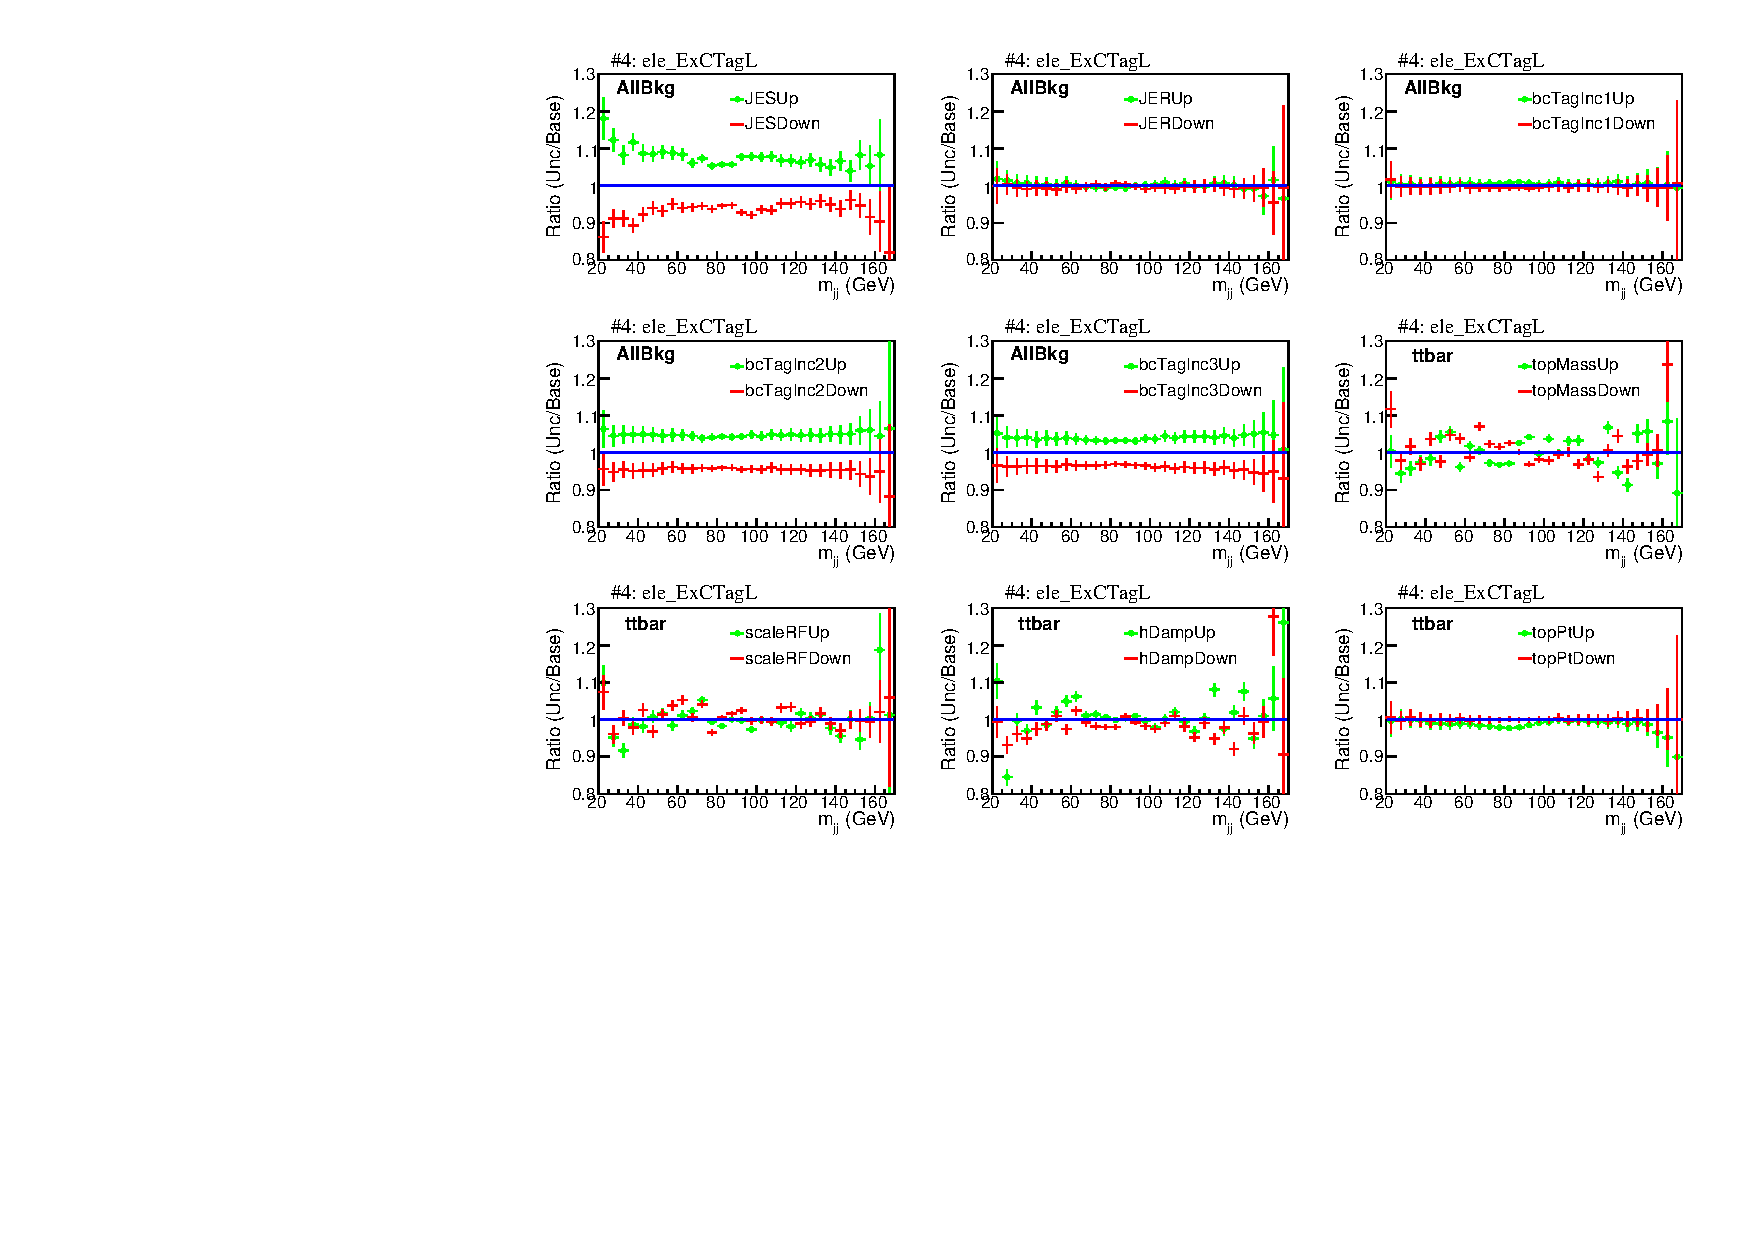
\includegraphics[width=0.80\linewidth]{Image/SYS/RatioBaseSys/mjj_4_ele_ExCTagL.pdf}}
    \caption{ Ratio of up and down with base template from exclusive loose charm category for \ejets channel.}
    \label{fig:shapeVslnN4}
\end{figure}
\begin{figure}
    \centering  
    {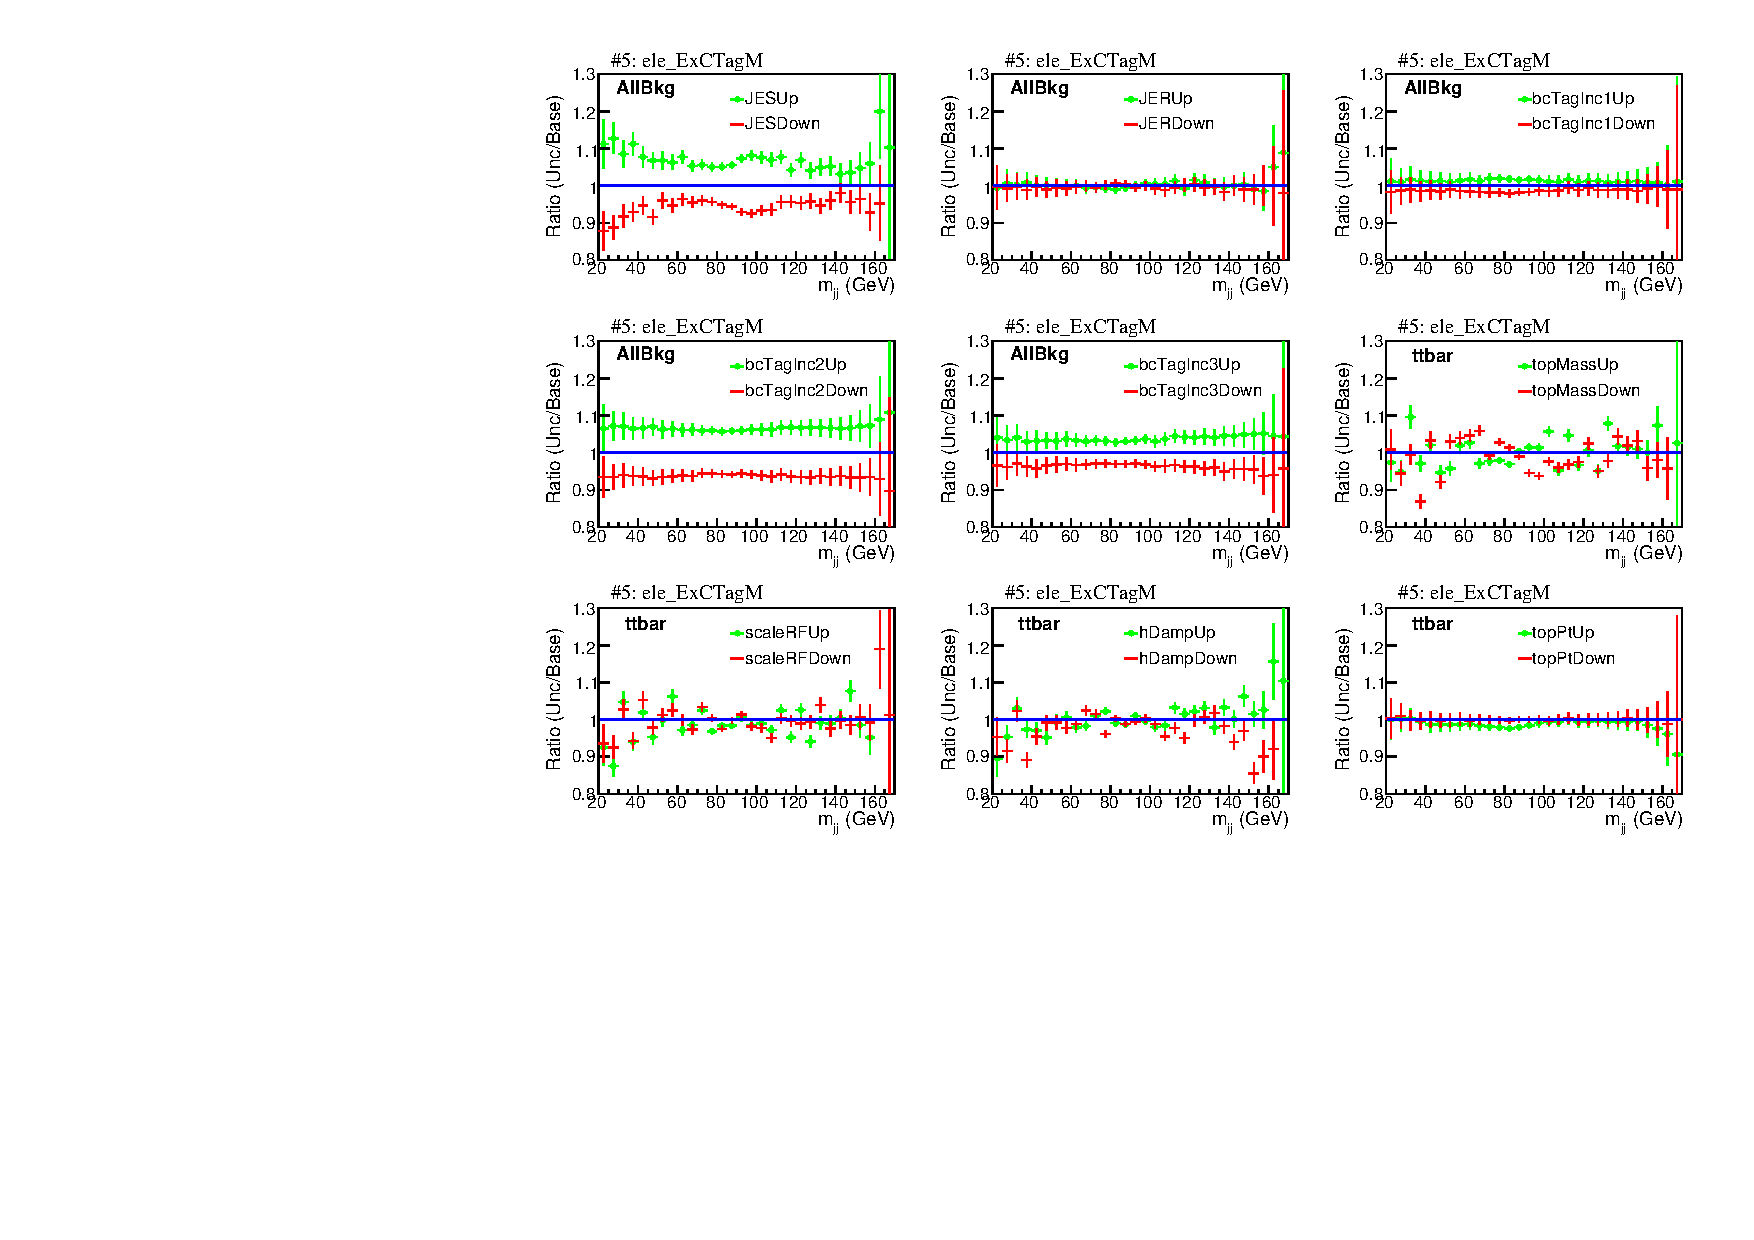
\includegraphics[width=0.80\linewidth]{Image/SYS/RatioBaseSys/mjj_5_ele_ExCTagM.pdf}}
    \caption{ Ratio of up and down with base template from exclusive medium charm category for \ejets channel. }
    \label{fig:shapeVslnN5}
\end{figure}


\begin{figure}
    \centering  
    {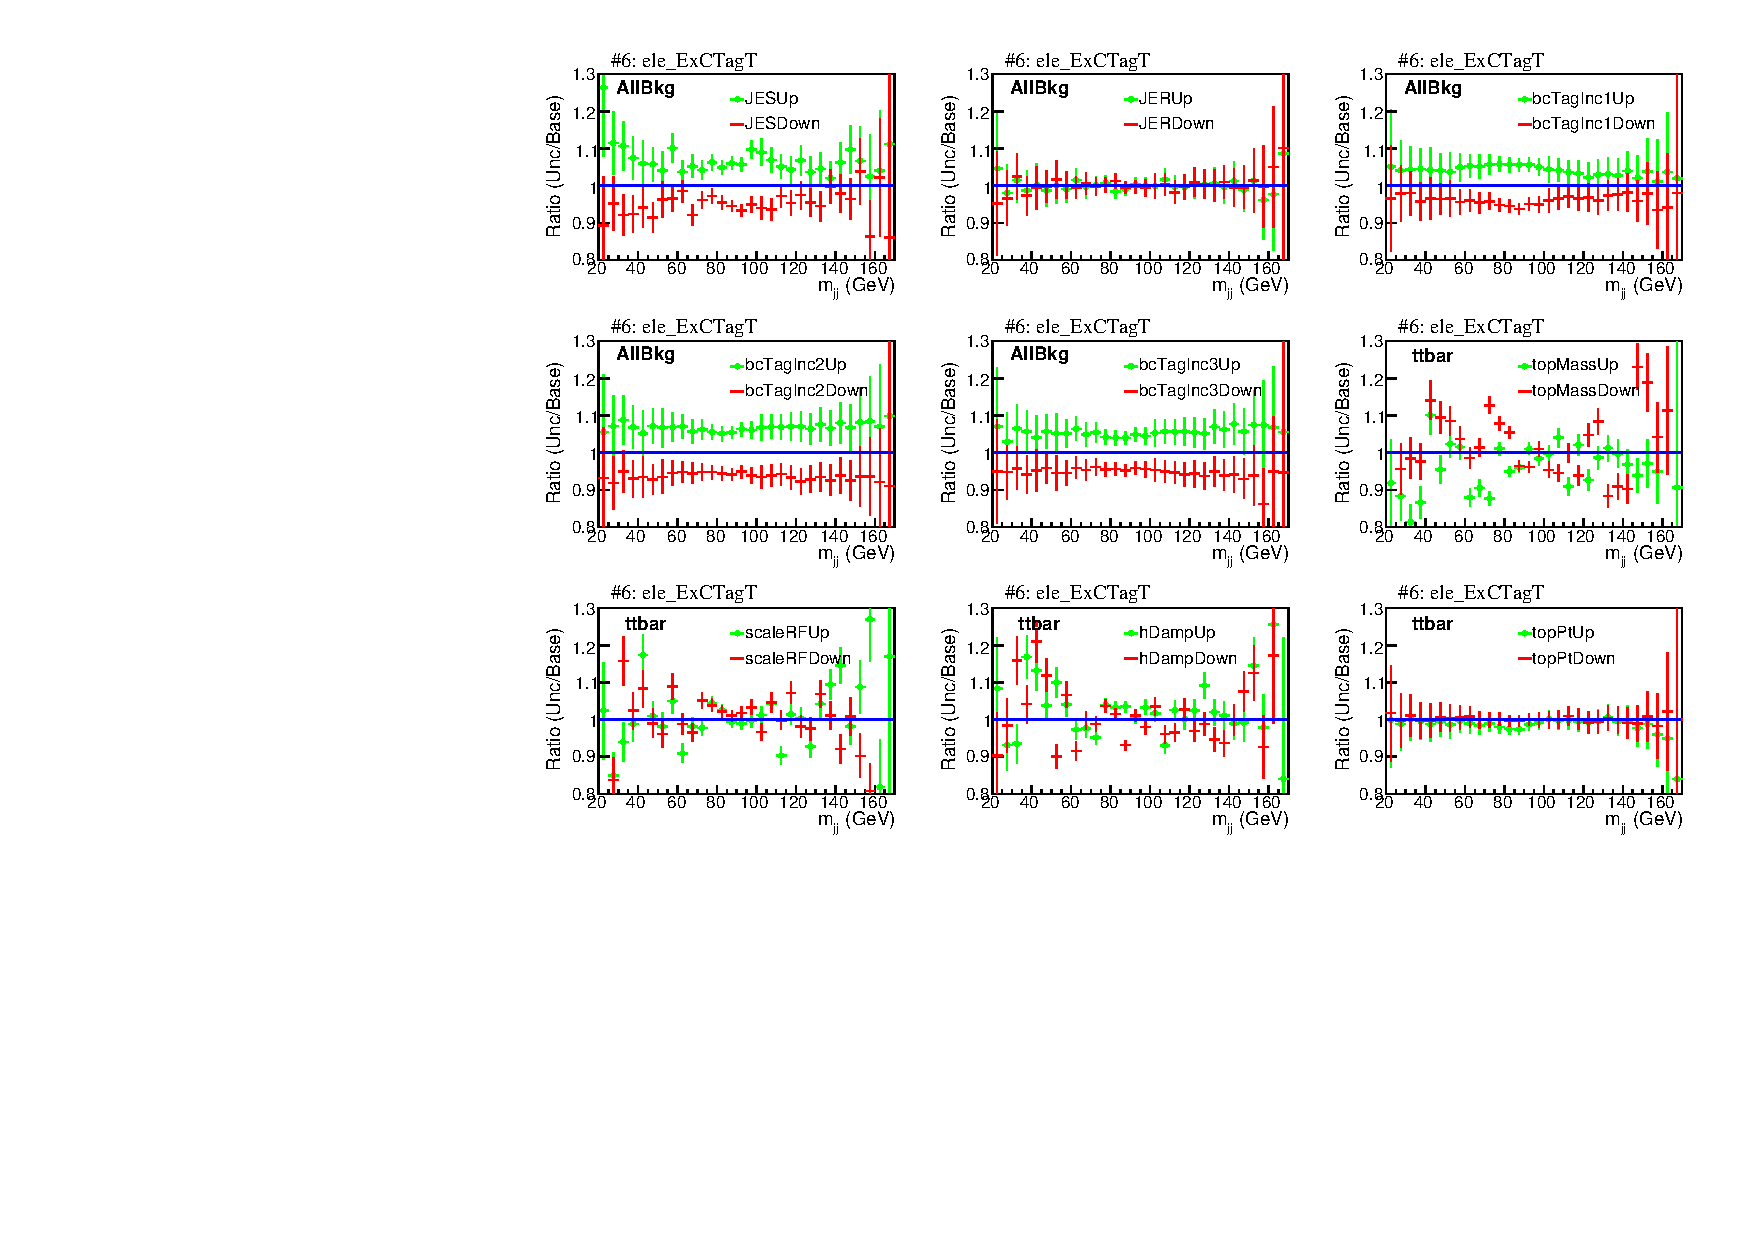
\includegraphics[width=0.80\linewidth]{Image/SYS/RatioBaseSys/mjj_6_ele_ExCTagT.pdf}}
    \caption{ Ratio of up and down with base template from exclusive tight charm category for \ejets channel.}
    \label{fig:shapeVslnN6}
\end{figure}

